% !TeX encoding = UTF-8
% !TeX program = pdflatex
% !TeX spellcheck = en-US

\documentclass[11pt]{article}

\usepackage[english]{babel}
\usepackage{graphicx}
\usepackage{listings}
\usepackage{xcolor}   % for \textcolor
\usepackage{tikz,pgfplots}
\usepackage[htt]{hyphenat}
\usepackage[hyphens]{url}
\usepackage{algorithm}
\usepackage{algpseudocode}
\usepackage{amsmath}
\usepackage{amssymb}
\MakeRobust{\Call}

\renewcommand{\algorithmicrequire}{\textbf{Input:}}
\renewcommand{\algorithmicensure}{\textbf{Output:}}


\title{Adversarial Examples on Malware Detection \\ {\large or just why you shouldn't use Neural Networks for Security Purposes} \\ - \\ Data Mining - Sapienza}
\author{Pietro Borrello - 1647357}
\date{\today}

\begin{document}

\maketitle

\tableofcontents
\newpage

\section{Introduction}
As widely known in the literature, machine learning algorithms, like deep neural networks, are in general susceptible to adversarial examples. It is possible to generate inputs, applying worst-case perturbations to existing ones, such that the crafted input is misclassified with high confidence \cite{adv-examples}. An adversarial example, given an input for a neural network (or any other ML model), is a perturbed version of the original one, such that preserves its functionalities and appears similar to the original, but is misclassified by the network. The problem arises in a large number of domain where neural networks are applied: for example, adversarial examples can be generated from images or speech, producing perfectly looking inputs undistinguishable on how they are perceived by humans, but that will be misclassified by the network.

\bigskip
In this paper we are going to investigate on how to produce adversarial examples in the case of Malware Detection. While when dealing with image or speech the goal is to apply small perturbations to the whole input not to change how it is perceived, when dealing with executable files, careful attention must be taken, since just a small modification to the binary values  (i.e. changing an offset or an opcode in the executable), leads to complete changes in functionalities. Therefore classical adversarial examples generation, is not suitable for our goal, and must be tuned. Our approach consisted in identifying which bytes in the malicious binary could be modified without changing its functionality, and how to map back these changes to the original binary, to produce a new malicious file, evading detection being classified as benign by the neural network. 

\section{Related Work}

\subsection{Adversarial Examples}
A great part of machine learning models have been shown to be vulnerable to manipulations of their inputs to produce adversarial examples. Adding a carefully chosen manipulation to craft a humanly indistinguishable new input against a target model, leads it to consistently misclassify the crafted input. This behaviour has been explained to be caused by the inherent linearity of the components of the model, even when the components result in a non-linear model, as in neural network \cite{adv-examples}. The goal of the misclassification can be targeted or un-targeted, depending on the fact whether the adversary chooses a particular class to produce the input to be misclassified into, or not. In case of binary classification both targeted and un-targeted attacks produce the same result.

When dealing with un-targeted attacks, different algorithms have been proposed. One of the first and simplest algorithms proposed is the {\tt Fast Gradient Sign Method}. Essentially, given an input $x$, it produces an adversarial example adding noise to the input itself to increase the loss function $L$ with respect to the predicted class $y$, computing:

$$
x^{adv} = x + \epsilon \cdotp sign(\nabla_{x} L(x, y_{pred}))
$$

with $L$ being the loss function, usually categorical cross entropy. While for targeted attacks, a slight modification of {\tt FGSM} is provided to decrease the loss for the input with respect to a target class:

$$
x^{adv} = x - \epsilon \cdotp sign(\nabla_{x} L(x, y_{target}))
$$

More advanced techniques have been proposed, but as we will se later, they won't suit our problem.
State of the art approach, have shown how adversarial examples can be transferable between models. It is shown how adversarial example, once crafted for a particular model trained on a particular dataset, remains misclassified with high probability, when analysed from both the same network trained on a different dataset, and from a different network trained on the same dataset. It has been shown also possible to generate an adversarial example in a black box fashion, without the knowledge neither of the underlying model, generating a synthetic dataset. 

\subsection{Malware Detection}  
The never ending cat and mouse game between malware writers and antivirus vendors, has seen an infinite list of techniques from both the parties. Any time malware detection system introduce a new method, a new malware evasion technique comes out from the hood to try to defeat the new method. As machine learning improves, neural networks seem the most promising step into precise malware detection, resilient to metamorphic code, or obfuscation techniques, producing encouraging results. 

Malware Detection through machine learning model, can be based either on feature extracted from the inspected binary, or on the raw bytes itself. Since malware producer, knowing which features are collected for the classification, could efficiently hide the malicious behaviour (has done for existing anti-antivirus techniques), the most promising ML technique to analyse malware seems to be the one based on raw bytes.

\section{The Problem}
Therefore we set our goal to produce Adversarial Examples against a neural network detector for Malware classification. This was guided to the hope in raising awareness on how neural network should not be trusted blindly for security purposes.

\subsection{The target Neural Network}
We took MalConv, that seems to be the state of the art for Malware Detection, to craft adversarial examples for \cite{eating}. The MalConv neural network detects Windows PE32 executable malware without any needing of preprocessing or feature selection. Therefore, crafting an adversarial example in this case, means directly changing bytes in the executable file.

\bigskip
The neural network structure is represented in the figure below:

\begin{center}
	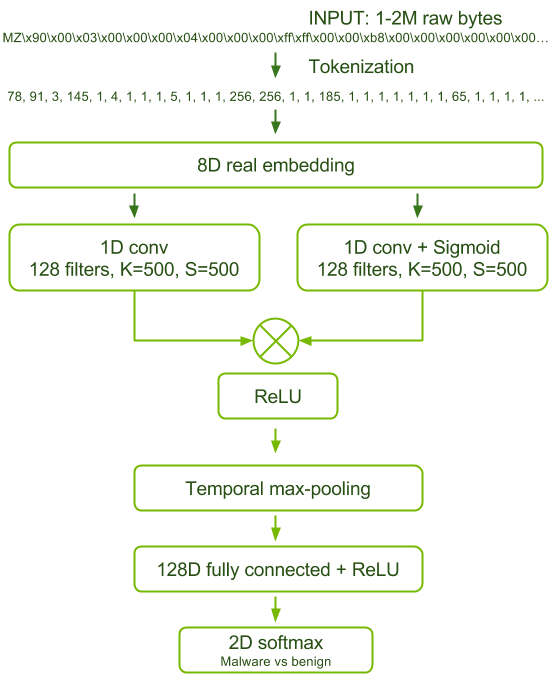
\includegraphics[width=0.5\textwidth]{malconv}
\end{center}

It takes the raw bytes from the executable files and maps each byte to a 8 dimensional floating point array. This is done to abstract the value of the bytes, that in the case of an executable file, simply means a data or an instruction, without having particular intensity or closeness meaning. The input dimension is fixed to 1MB due to resources contraint, bigger file are cropped, while smaller files are padded to match the dimension.
The convolutional layers are used to tackle local spatial relations, as can be malicious functions or data. The network produces a binary classification value, stating if it believes or not the file analysed to be a malware. 

\subsection{Challenges}
There exists multiple challenges to craft an adversarial example for such a problem. First of all, as previously stated, our adversarial input must be a valid PE32 executable, therefore bytes in the original file must be changed paying attention not to destroy malicious functionality. Additionally the network itself poses challenges to the creation of adversarial examples: the presence of the embedding layer to translate bytes values into 8 dimensional vector, makes all the existing algorithms not applicable as they are. In fact they usually require to compute the gradient of the loss of the output class, with respect to the input, but the embedding layer at the beginning of the network makes the whole network not differentiable. We will tackle the different challenges separately.

\subsection{Windows PE32 Format}
To understand how to deal with the executable files that are given in input is useful to know in some detail the layout of the Portable Executable file format for the Windows operating system. 

A Windows binary begins with the DOS header. This is placed at the beginning for legacy reasons, and the Windows loader, when executing a program, first checks if the first two bytes of the file match the MS-DOS signature {\tt MZ}, to indicate a valid executable format. It then reads 4 bytes from the offset {\tt 0x3c} to know the location of the PE header, while ignoring the remaining bytes of the DOS header and the DOS stub (they contain a valid MS-DOS program to be executed if no PE header found). 

\bigskip
The PE header contains important metadata on which Windows subsystem can run the file, and how. Such header includes information as the entry point of the program, along with the sections the program will be composed by, with they respective metadata. Each program will be composed by multiple sections that may contain code, data or resources, each of the section must start at an offset that is aligned to at least $512$ bytes in the file, or more, if stated in the header. Padding of zero bytes is present to make the sections align properly. 

The figure below illustrates the headers structure:

 \begin{center}
	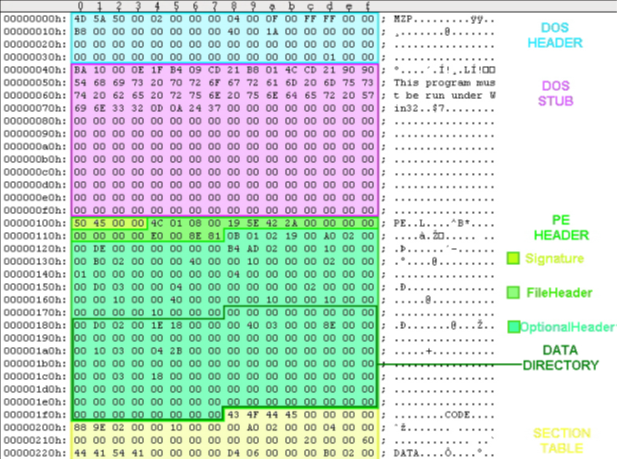
\includegraphics[width=0.7\textwidth]{pe_format}
\end{center}

\section{Design Choices}

\subsection{Choosing bytes to modify}
The first design choice that we had to make, was deciding how to change the provided malware, to make it an adversarial example, preserving its functionalities. An analysis of the PE format, provided us with some candidates bytes to be changed. As stated in the previous chapter, the DOS header is completely ignored by the windows loader, if it finds two valid bytes in the MS-DOS signature and 4 valid bytes at the offset {\tt 0x3c}. Therefore the whole DOS header, apart from the previously mentioned bytes, can be changed along with the DOS stub, without modifying the functionalities of the malware. While we could have been fine tuning our choices in the header bytes to change, including some bytes in the PE header (like for example the compilation timestamp or reserved bytes that are present but not used), we decided to leave them unchanged, to avoid to tide us into architecture version specific details. 

In addition to the DOS header bytes, we included in the set of bytes to be mutable, also the padding bytes between sections. They are present in the executable image only to make the section starting points to be aligned to 512 bytes boundaries, and are never accessed by the software. Therefore any change to those bytes, will pass unnoticed with respect to binary functionality. We opted out changing data in the malware, like strings in the executable. This was because, even if changing them wouldn't have changed the binary functionality, it could have impacted on how the malware could have been perceived by the victim (i.e. strings describing instruction to pay a ransom in a Ransomware), so leaving them unchanged was a safe default behaviour.

All the bytes described above, gave us around less than the 1\% of the bytes of the executable file to be changed, that was still enough to mount our attack.

\subsection{Facing the embedding layer Problem}
While inserting an embedding layer in the network, boosted the accuracy for malware detection, this was a challenging wall to break in order to mount the attack. Being non differentiable, the embedding layer, doesn't allow to compute the gradient of the loss, with respect to the input. Therefore since most of the existing attacks that are based on gradient descent, are not applicable to our case as they are. Following the solution proposed by \cite{maladv}, we choose to compute the loss, to apply existing methods, with respect to the output of the embedding layer itself to avoid differentiation problems. Therefore, instead of obtaining an adversarial input, the output of our algorithm would be an adversarial embedding. 

Then the problem is how to map the produced adversarial embedding to valid bytes to get back a new executable file, since in the produced adversarial embedding, for the modified vectors there won't exist any byte that would match the particular vector once passed into the layer. In fact the embedding layer maps 256 possible bytes to 256 possible 8 dimensional real vectors, and once modified there won't be low chance to match exactly any other existing vector. 

The approach we took was to try to map each 8 dimensional vector to its nearest neighbour in the 8 dimensional space, and then taking the corrispective byte back. The process of taking the nearest neighbour approximates the solution found by the algorithm, but this was enough to build the attack. 

\subsection{Tuning existing algorithms}
All the existing algorithm to construct adversarial examples, are focused on making imperceptible changes on the input, to make it be misclassified by the network. This produces perfectly looking inputs undistinguishable by human perceptions. What differs from our goal is that we are not interested on making changes imperceptible for humans, but we only need to preserve malware functionality, avoiding changing meaningful bytes. While it doesn't seem a problem, complications indeed arises when applying these existing algorithm to the embedding layer as we designed. 

In fact, since we have to map back the adversarial embedding layer to actual bytes using nearest neighbours, when applying such imperceptible changes to the embedding vectors, what we obtain is that the nearest neighbour of the adversarial embedding vectors are with high probability the original embedding vectors themself, resulting in less or no change at all in the input file. Given that the perturbations that we applied where far bigger than the one recommended in state of the art techniques, to be sure, that, when computing the input with respect to the embedding, we would obtain an adversarial example with high probability. 

Therefore we had to discard existing algorithms that rely on minimisation problems to get a small perturbation \cite{carlini}, and we developed a slight modification of the targeted Fast Sign Gradient Method, by empirically tuning the steps to obtain adversarial example with highest probability possible. 

We are not stating that the modification to the {\tt FSGM} could generalise to other problems, but the following algorithm was what worked in practice, producing adversarial examples reliably:

\begin{algorithm}
\caption{Fast Gradient Descent Approximation}
\begin{algorithmic}[1]
  \Require $X$: executable, $mask$: editable bytes mask, $y$: target
  \Ensure $X^{adv}$ : $X$ adversarial example classified as $y$
  \State $X^{adv} \gets \bot$
  \State $Z \gets \Call{Emb}{X}$
  \State $Z^{adv} \gets Z$

  \Repeat
  \State $g \gets \Call {MaxAbsScale}{mask \times \nabla_{Z^{adv}} L(Z^{adv}, y)}$
  \State $Z^{adv} \gets Z^{adv} - g$
  \Until $Z^{adv}$ classified as $y$ with high confidence
  
  \ForAll{$z^{adv}_{i} \in Z^{adv}$}
  \State $x^{adv}_{i} \gets \Call{Emb$^{-1}$}{\Call{NearestNeighbour}{z^{adv}_{i}, \Call{Emb}{X}}}$
  \EndFor
  \State \Return $X^{adv}$
\end{algorithmic}
\end{algorithm}

\section{Implementation}
We decided to implement the whole process using the {\tt Keras} deep learning library. We collected 302 malwares from the hood to be classified, on top of which construct adversarial examples. 

\begin{thebibliography}{99}
	\bibitem{adv-examples}
		Explaining and Harnessing Adversarial Examples,
		Ian J. Goodfellow, Jonathon Shlens, Christian Szegedy,
		arXiv:1412.6572
	\bibitem{black-box}
		Practical Black-Box Attacks against Deep Learning Systems using Adversarial Examples, 
		Nicolas Papernot, Patrick McDaniel, Ian Goodfellow,
		2016
	\bibitem{eating}
		Malware Detection by Eating a Whole EXE,
		Edward Raff, Jon Barker, Jared Sylvester,
		arXiv:1710.09435
	\bibitem{maladv}
		Adversarial Examples on Discrete Sequences for Beating Whole-Binary Malware Detection,
		Shir Aviv Reuven, Joseph Keshet,
		arXiv:1802.14528v1
	\bibitem{carlini}
		Towards Evaluating the Robustness of Neural Networks,
		Nicholas Carlini, David Wagner,
		arXiv:1608.04644v2
		
\end{thebibliography}

\end{document}










